\subsection{Details of Fig.\,\ref{fig:PL}}

\paragraph{Target} We consider a two-layer structured RF teacher, with feature map
\begin{align}
    \varphi_*(x)=\mathrm{tanh}\left(
    W_*x
    \right)
\end{align}
where the weight $W_*=Z_*\Tilde{C}_1^{\frac{1}{2}} \in\mathbb{R}^{d\times d}$ has covariance
\begin{align}
    \Tilde{C}_1=\mathrm{diag}(\{k^{-0.3}\}_{1\le k\le d}).
\end{align}

\paragraph{Student} We consider the task of learning this target with a four-layer RF student, with feature map
\begin{align}
    \varphi(x)=\tanh W_3(\tanh\left(
    W_2\tanh(W_1x)
    \right))
\end{align}
where, in order to introduce inter-layer and target/student weight correlations, we considered $W_2=W_1$, with
\begin{align}
    W_1=\frac{1}{2}Z_1\mathrm{diag}(\{k^{-\frac{\gamma}{2}}\}_{1\le k\le d})+\frac{1}{2}W_*,
\end{align}
for $\gamma\in\{0.0,0.2,0.5,0.8\}$. In other words, the covariance $C_1$ of $W_1,W_2$ is a sum of two power laws with decay $\gamma$ and $0-3$. Finally, in order to introduce another form of correlation, we chose
\begin{align}
    W_3=Z_3 C_3^{\frac{1}{2}}
\end{align}
where the covariance $C_3$ depends on the previous weights as
\begin{align}
C_3=(W_1W_1^\top +\frac{1}{2}\mathbb{I}_d)^{-1}.
\end{align}


\subsection{MNIST Experiments}
\label{app:real_data}
\paragraph{Data set}
We use the MNIST data set which we normalize by pixel-wise centering and global scaling to ensure unit variance. For each normalized image $x_i\in\R^{784}$ we define a label
\[y_i := \begin{cases} 1,&  \text{ if }x_i\text{ is an even digit,}  \\ -1,& \text{ if }x_i\text{ is an odd digit.}\end{cases}
\]
We split the data set into four parts:
\begin{itemize}
\item[$10\%$] Test data $I_\mathrm{test}$ 
\item[$25\%$] Training data for the Adam optimizer $I_\mathrm{Adam}$,
\item[$25\%$] Training data for regression $I_\mathrm{reg}$,
\item[$40\%$] Data for approximating the (empirical) population covariance $I_\mathrm{emp}$.
\end{itemize}


\paragraph{Neural network}
We then train a simple neural network of the form 
\begin{equation}
    \begin{aligned}
    &x\mapsto \theta^\top\varphi(x), \quad \varphi(x):=\theta^\top\operatorname{relu}(W_2 \operatorname{relu}( W_1 x)), \text{ where } \\
    &W_1\in\R^{2352\times 784},\quad W_2\in\R^{2352\times 2352}, \quad \theta\in\R^{2352}
    \end{aligned}
\end{equation}
using the Adam optimizer over $120$ epochs with a batch size of $128$ using only the $I_\mathrm{Adam}$ split. During training we save the \emph{feature maps} $\varphi_t$ at various time steps $t$ in order to study the training dynamics. 

\paragraph{Feature ridge regression} We then perform a ridge regression task using the features $\varphi_t(x_i)$ by minimizing
\begin{equation}
    \theta(t,\lambda,I):=\arg\min_\theta \Bigl(\frac{1}{\abs{I}}\sum_{i\in I} (y_i- \theta^\top\varphi_t(x_i))^2 + \lambda \norm{\theta}^2\Bigr)
\end{equation}
for various random subsets $I\subset I_\mathrm{reg}$, and $I_\mathrm{test}$, empirically estimate the \emph{generalization error} 
\begin{equation}
    \mathcal E_\mathrm{gen}(t,\lambda,I)^2 := \frac{1}{\abs{I_\mathrm{test}}} \sum_{i\in I_\mathrm{test}} (y_i - \theta(t,\lambda,I)^\top\varphi_t(x_i))^2.
\end{equation}

\paragraph{Deterministic equivalent}
In order to compare $\mathcal E_\mathrm{gen}(t)$ with the theoretical prediction from~\Cref{thm genRMT informal}, we need to determine the covariance of the features $\phi_t$ as well as the label-feature covariance and the label variance. 
To do so, we use the $I_\mathrm{emp}$ part of the data to empirically estimate 
\begin{equation}
    \begin{aligned}
    \Omega_t&:=\frac{1}{\abs{I_\mathrm{emp}}}\sum_{i\in I_\mathrm{emp}} \varphi_t(x_i)\varphi_t(x_i)^\top\in\R^{2352\times2352}, \\
    \psi_t&:=\frac{1}{\abs{I_\mathrm{emp}}}\sum_{i\in I_\mathrm{emp}} \varphi_t(x_i)y_i\in\R^{2352}, \\
    \sigma^2&:= \frac{1}{\abs{I_\mathrm{emp}}}\sum_{i\in I_\mathrm{emp}} y_i^2\in \R,
    \end{aligned}
\end{equation}
and note that we expect this to be a reasonable approximation since $\abs{I_\mathrm{emp}}=27805\gg 2352$. Using these we have the formula 
    \begin{equation}\label{eq Egen rmt2}
            \mathcal E_\mathrm{gen}^\mathrm{rmt}(t,\lambda,n): = \frac{ \sigma^2 -  n\lambda m_t\psi_t^\top (M_t+\lambda M_t^2)\psi_t }{1-n(m_t\lambda)^2\Tr \Omega_t M_t\Omega_t M_t}
    \end{equation}
analogous to~\Cref{eq Egen rmt}, where $m_t,M_t=m_t(\lambda,n),M_t(\lambda,n)$ are the solution to 
\begin{equation}
    \begin{aligned}
    \frac{1}{m_t(\lambda,n)} &= \lambda + \Tr \Omega_t (1 + n m_t(\lambda,n)\Omega_t )^{-1}, \\
    M_t(\lambda,n) &:= (\lambda + \lambda n m(\lambda,n)\Omega_t )^{-1}.
    \end{aligned}
\end{equation}

We observe in~\Cref{fig:real_emp} that $\mathcal E^\mathrm{rmt}_\mathrm{gen}$ is indeed an excellent approximation for $\mathcal E_\mathrm{gen}$ throughout the training and for various choices of regularization. In~\Cref{fig:real_det} we depict the interesting dynamics of the learning curves throughout the training process with a significant shift of the interpolation threshold to the left. 
\begin{figure}[ht]
    \centering
    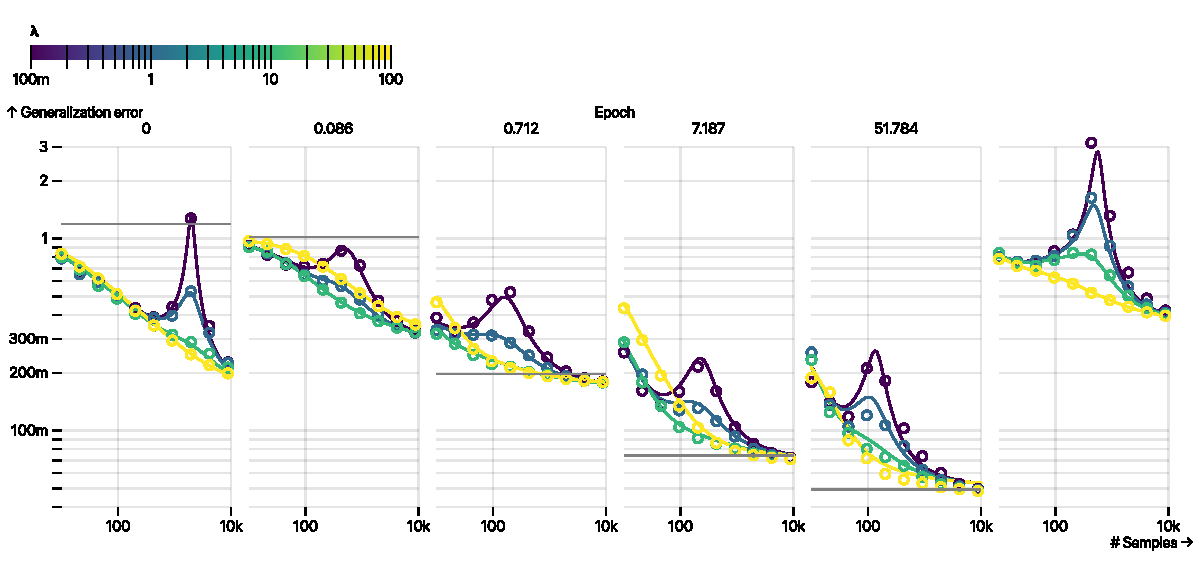
\includegraphics[width=\linewidth]{chapters/deeprf/figs/real_emp.pdf}
    \caption{Plot of $\mathcal E^\mathrm{rmt}_\mathrm{gen}$, $\mathcal E_\mathrm{gen}$ for various regularization parameters $\lambda$ and time steps $t$ (in ``epoch.step'' format). The horizontal lines represent the generalization error of the neural network, the curves $\mathcal E^\mathrm{rmt}_\mathrm{gen}$ and the dots $\mathcal E_\mathrm{gen}$. The last pane contains a linear regression model for the sake of comparison. Interestingly, for this particular case already the random feature model outperforms linear regression.}
    \label{fig:real_emp}
\end{figure}
\begin{figure}[ht]
    \centering
    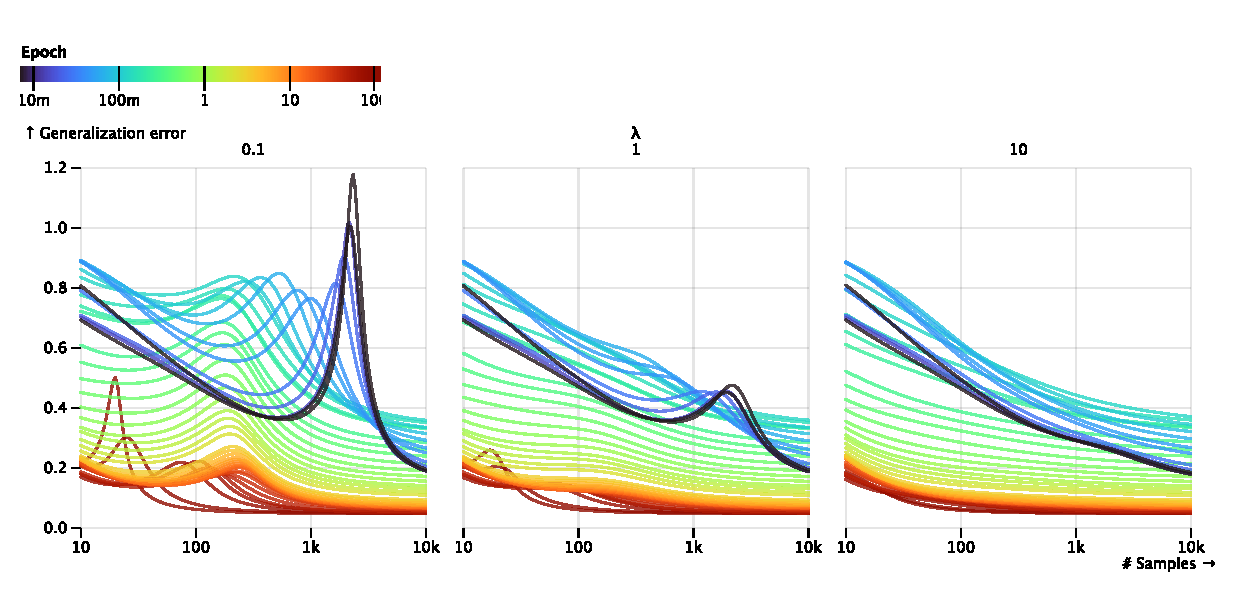
\includegraphics[width=\linewidth]{chapters/deeprf/figs/real_det.pdf}
    \caption{Dynamics of $\mathcal E^\mathrm{rmt}_\mathrm{gen}$ throughout the training}
    \label{fig:real_det}
\end{figure}

\paragraph{Optimal regularization}
So far we have focused on fixed regularization parameters. Using the deterministic equivalent we can also find the optimal regularization parameter \begin{equation}
    \lambda_\mathrm{opt}(t,n) := \arg\min_\lambda \mathcal E_\mathrm{gen}^\mathrm{rmt}(t,\lambda,n) 
\end{equation} 
for each sample complexity $n$ and time $t$ by simply one-dimensional minimization. In~\Cref{fig:real_opt} we show the corresponding results. Interestingly ridge regression initially performs worse than the random feature regression also at optimal regularization. Then in the initial phase of training the performance of feature regression deteriorates before improving way beyond the initialization performance.   
\begin{figure}
    \centering
    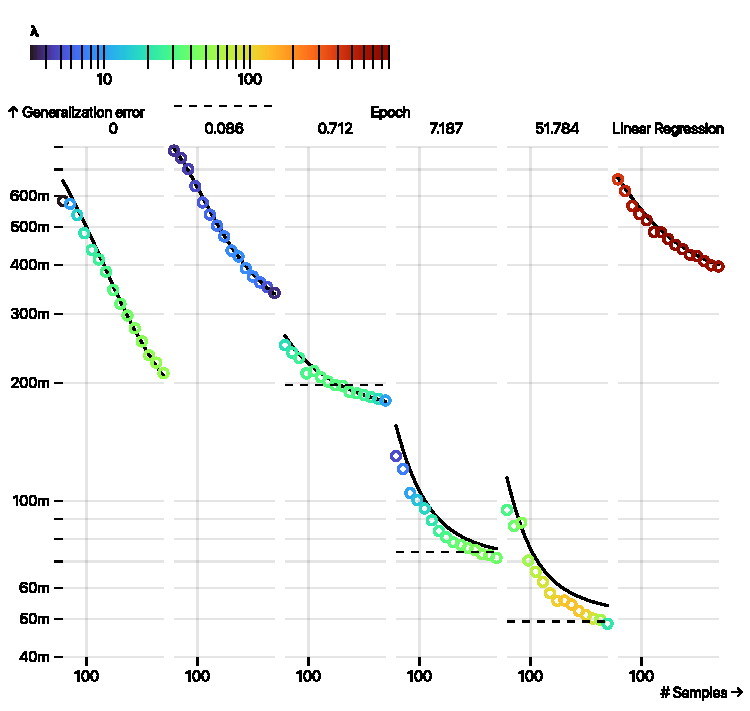
\includegraphics[width=.6\linewidth]{chapters/deeprf/figs/real_opt_emp.pdf}
    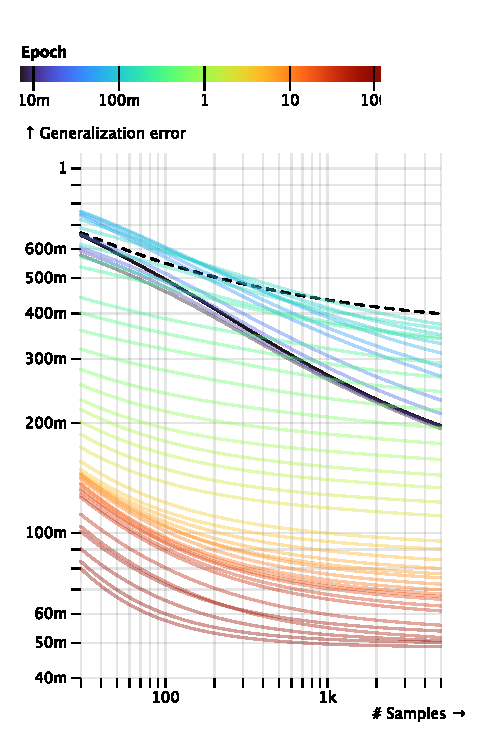
\includegraphics[width=.37\linewidth]{chapters/deeprf/figs/real_opt_det.pdf}
    \caption{The left pane shows $\mathcal E_\mathrm{gen}$ and $\mathcal E_\mathrm{gen}^\mathrm{rmt}$ throughout the training process at \emph{optimal} regularization $\lambda_\mathrm{opt}$. The colour of the dots encodes the value of $\lambda_\mathrm{opt}$, while the dashed lines represent the generalization error of the neural network. The right pane shows the dynamics of $\mathcal E_\mathrm{gen}^\mathrm{rmt}$ throughout the training process, compared with linear regression.}
    \label{fig:real_opt}
\end{figure}

\subsection{Synthetic MNIST experiments}\label{synth MNIST}
We carried out similar experiments for synthetic data in order to empirically study the effect of population covariance linearization. 

\paragraph{Data}
We generate Gaussian random vectors of zero mean and variance matching the variance of the normalized MNIST images described above. The synthetic labels are generated by a one hidden layer random feature network 
\[ \varphi_\ast(x):= \theta_\ast \tanh(W_\ast x), \quad W_\ast\in\R^{800\times 784}, \theta_\ast\in\R^{800} \]
for fixed but random $W_\ast,\theta_\ast$. 

\paragraph{Neural network}
We again train a simple neural network of the form 
\begin{equation}
    \begin{aligned}
    &x\mapsto \theta^\top\varphi(x), \quad \varphi(x):=\theta^\top\operatorname{relu}(W_2 \operatorname{relu}( W_1 x)), \text{where }\\
    &W_1\in\R^{800\times 784},\quad W_2\in\R^{700\times 800}, \quad \theta\in\R^{700}
    \end{aligned}
\end{equation}
using the Adam optimizer over $50$ epochs with a batch size of $128$ using $40\ 000$ samples. During training we save the \emph{feature maps} $\varphi_t$ at various time steps $t$ in order to study the training dynamics. 

\paragraph{Feature ridge regression} We perform feature ridge regression on the trained features $\varphi_t$ exactly as described above. The fact that the labels are now generated by a feature model now enables us to test the effect of population covariance linearization. In~\Cref{fig:art-lin} we observe that for random features the linearized deterministic equivalent is an excellent approximation for the empirically observed feature ridge regression error. However, during training the prediction deteriorates. We suspect that this effect is due to outlying eigevalues of the weight matrices which increasingly violate~\Cref{corr rainbow}.  

\begin{figure}
    \centering
    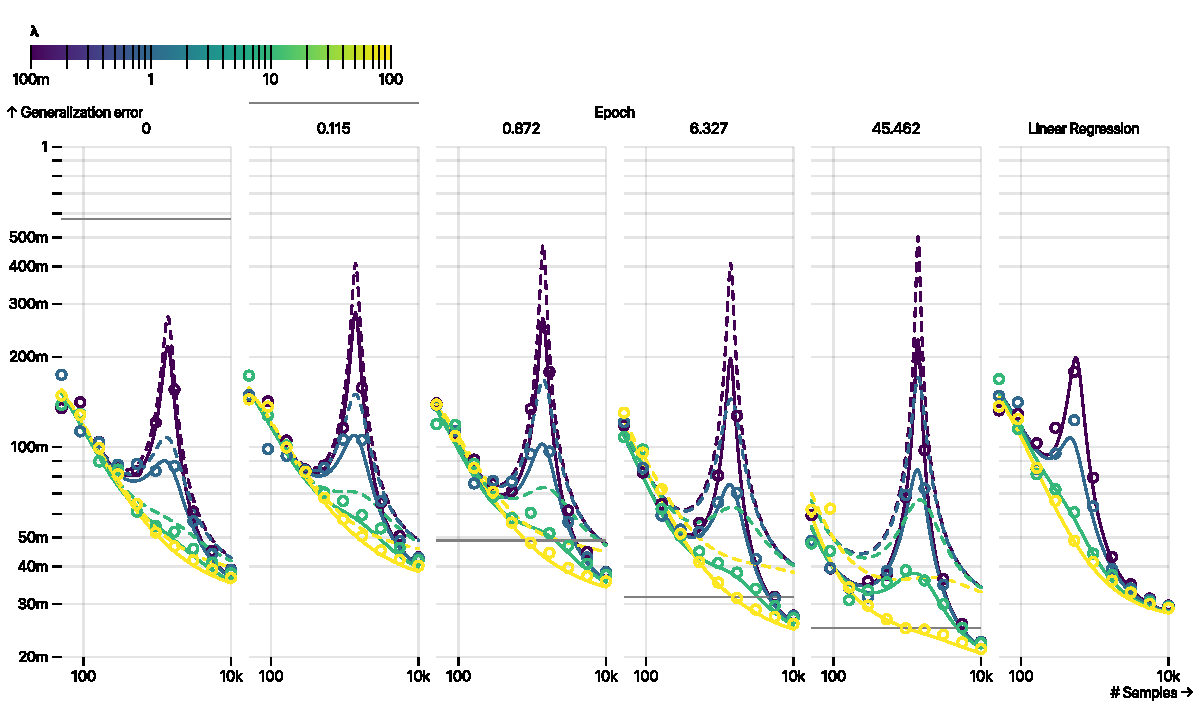
\includegraphics[width=\linewidth]{chapters/deeprf/figs/art_emp.pdf}
    \caption{The solid and dashed lines represent $\mathcal E_\mathrm{gen}^\mathrm{rmt}$ using the empirical population covariances and the linearized population covariances, respectively. The dots represent the empirical $\mathcal E_\mathrm{gen}$ while the horizontal line show the test error of the neural network during training. The right-most pane shows linear regression for comparison.}
    \label{fig:art-lin}
\end{figure}
